\subsection{Progettazione architetturale}
Il periodo di progettazione architetturale comincia il 2019-02-01 e si conclude il 2019-03-15. L'inizio coincide con il giorno successivo alla conclusione del Consolidamento dei Requisiti. La conclusione coincide con con la consegna dei documenti per la Revisione di progettazione. \\
\subsubsection{Incrementi}
In questo periodo si effettuano 3 incrementi e le attività principali sono:
\begin{itemize}
	\item \textbf{Correzione e Verifica:} si inizia correggendo e verificando i documenti precedentemente presentati (Norme di progetto, Piano di progetto, Piano di qualifica e Analisi dei requisiti) in base alle indicazioni ricevute dalla Revisione dei Requisiti. Inoltre si migliora e si aggiorna il documento contenente il \textit{Glossario};
	\item \textbf{\gl{Technology Baseline}:} in questa attività vengono studiate ed analizzate le scelte tecnologiche, tra cui le possibili librerie da utilizzare per lo sviluppo del prodotto. Verranno quindi decisi i design pattern da utilizzare nella creazione del prodotto e l'architettura generale del software.
\end{itemize}

\subsubsection{Progettazione architetturale - Gantt delle attività}

\begin{figure} [H]
	\centering
	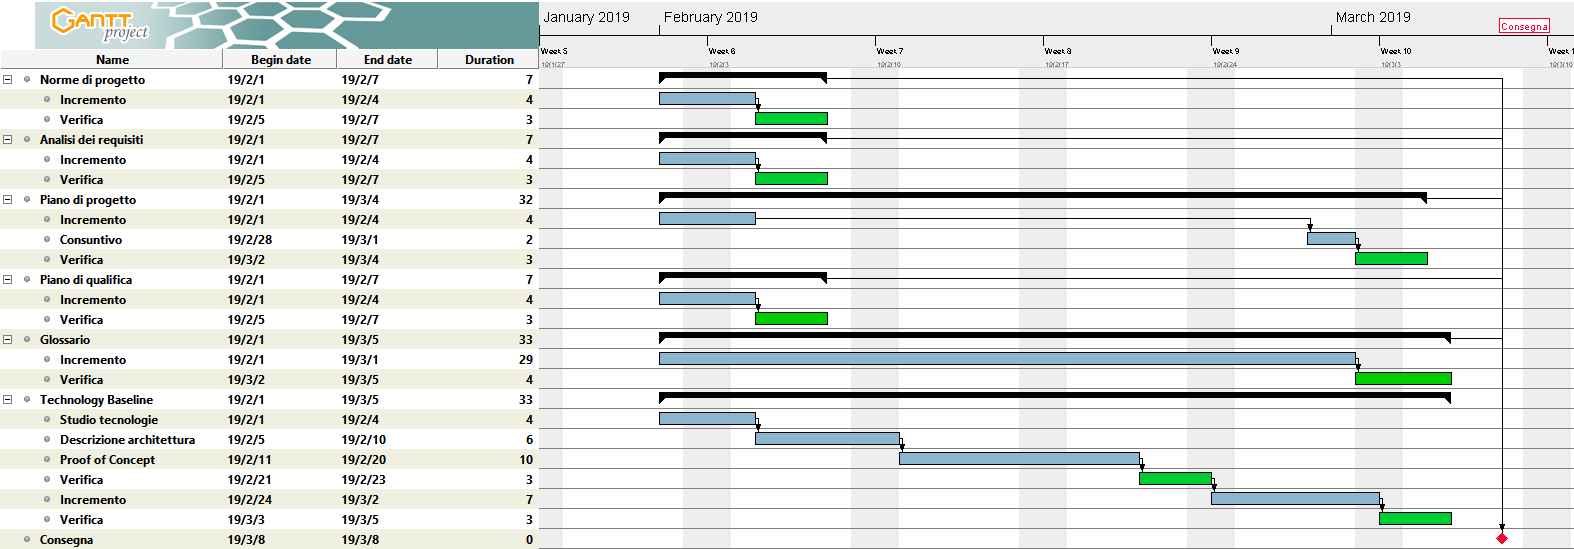
\includegraphics[scale=0.3]{Res/Gantt/Progettazione}
	\caption{Diagramma dei casi d'uso}\label{}
\end{figure}

\pagebreak
